\documentclass[12pt]{beamer}

%CORE PACKAGES---------------------------------
\usepackage{amsmath, amssymb, graphicx, booktabs, tabularx, setspace, soul}
\usepackage{subcaption}
\usepackage{tikz, pgfplots}
\pgfplotsset{compat=1.18}
\usetikzlibrary{positioning, arrows.meta, arrows.meta, positioning, shapes, calc}
\usepackage[many]{tcolorbox}
\usepackage[ruled,vlined]{algorithm2e}
\usepackage{minted}

%FONTS & STYLING-------------------------------
\usepackage{fontspec, emoji, tikzsymbols}
\usefonttheme{professionalfonts}
\setsansfont[
UprightFont     = *Light,
BoldFont        = *Bold,
ItalicFont      = *Light Italic,
BoldItalicFont  = *Bold Italic,
Ligatures       = TeX,
Scale           = MatchLowercase
]{Frutiger LT Pro}
\renewcommand{\familydefault}{\sfdefault}
\linespread{1.}\selectfont
\hyphenpenalty=10000
\exhyphenpenalty=10000

%COLORS & THEMES-------------------------------
\definecolor{aggiemaroon}{RGB}{80,0,0}
\definecolor{beamer@blendedblue}{RGB}{80,0,0}
\definecolor{AggieMaroon}{HTML}{500000}
\definecolor{SoftGray}{HTML}{F5F5F5}
\definecolor{DarkGray}{HTML}{333333}
\definecolor{AccentBlue}{HTML}{2F5597}
\usecolortheme{default}

\setbeamertemplate{itemize items}{•}
\setbeamertemplate{itemize subitem}[•]
\setbeamertemplate{itemize subsubitem}[•]
\renewcommand{\UrlFont}{\ttfamily\footnotesize}
\newcommand{\vocab}[1]{\textcolor{AggieMaroon}{\textbf{#1}}}
\newcommand{\question}[1]{\begin{block}{Question}#1\end{block}}
\newcommand{\smallnote}[1]{{\footnotesize\textcolor{DarkGray}{#1}}}

%HYPERLINKS------------------------------------
\usepackage{hyperref}
\hypersetup{
colorlinks=true,
linkcolor=aggiemaroon,
urlcolor=aggiemaroon,
citecolor=aggiemaroon
}

%BEAMER TEMPLATES------------------------------
\setbeamertemplate{caption}[numbered]
\setbeamertemplate{navigation symbols}{}
\setbeamertemplate{footline}{
\color{aggiemaroon}{\hfill \insertframenumber/\inserttotalframenumber \hspace{2pt} \vskip2pt}
}

%CUSTOM ENVIRONMENTS---------------------------
\newenvironment{stepenumerate}{
\begin{enumerate}[<+->]
}{\end{enumerate}}

\newenvironment{stepitemize}{
\begin{itemize}[<+->]
}{\end{itemize}}

\newenvironment{stepenumeratewithalert}{
\begin{enumerate}[<+-| alert@+>]
}{\end{enumerate}}

\newenvironment{stepitemizewithalert}{
\begin{itemize}[<+-| alert@+>]
}{\end{itemize}}

%DOCUMENT INFO----------------------------------
\title{Decision and Risk Analysis}
\subtitle{Lecture 2: \textbf{Bayes’ Rule}}
\author{\emph{}}
\date{\color{aggiemaroon}{
DAEN 427/ISEN 427/ISEN 627\\
\textbf{Alexander Abuabara}\\
Fall 2026
}}
\titlegraphic{\vfill 
\includegraphics[height=1.2cm]{TAMU_logo.png}}

%-----------------------------------------------
\begin{document}

%-----------------------------------------------
\maketitle

%-----------------------------------------------
\begin{frame}{}
\centering
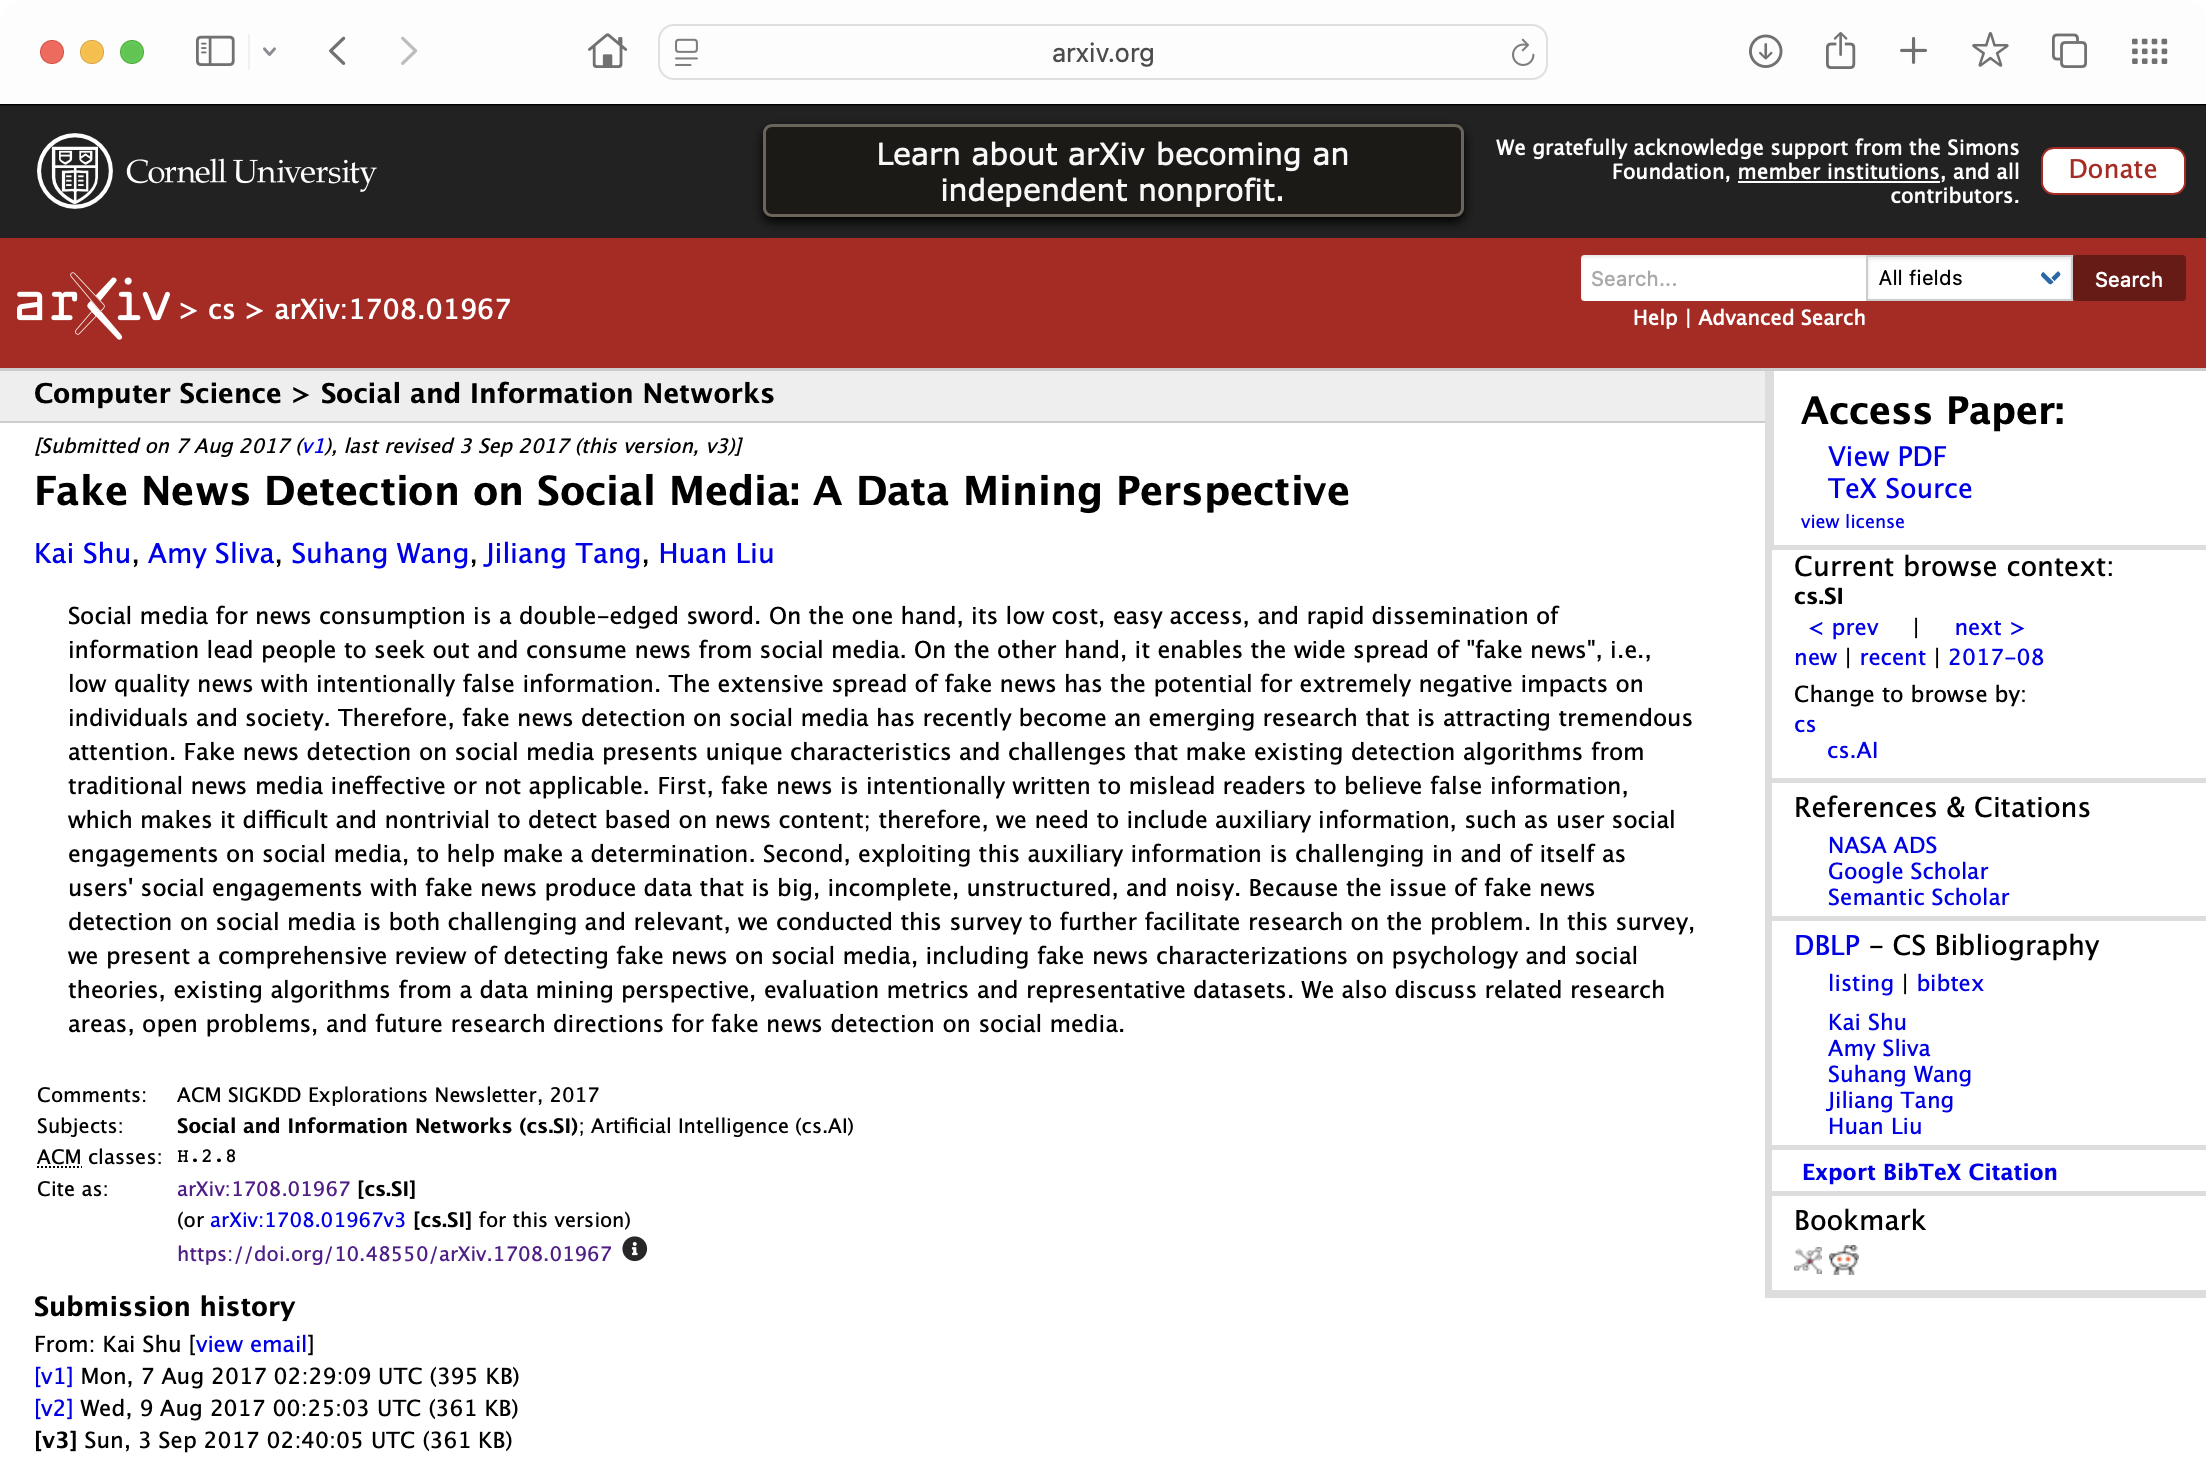
\includegraphics[height=.75\textheight]{Screenshot 2026-05-22 at 5.13.47 PM}
{\footnotesize \url{https://arxiv.org/abs/1708.01967} for details.}
\end{frame}

%-----------------------------------------------
\begin{frame}{}
\begin{block}{Framework}
\vspace{.4cm}
\centering
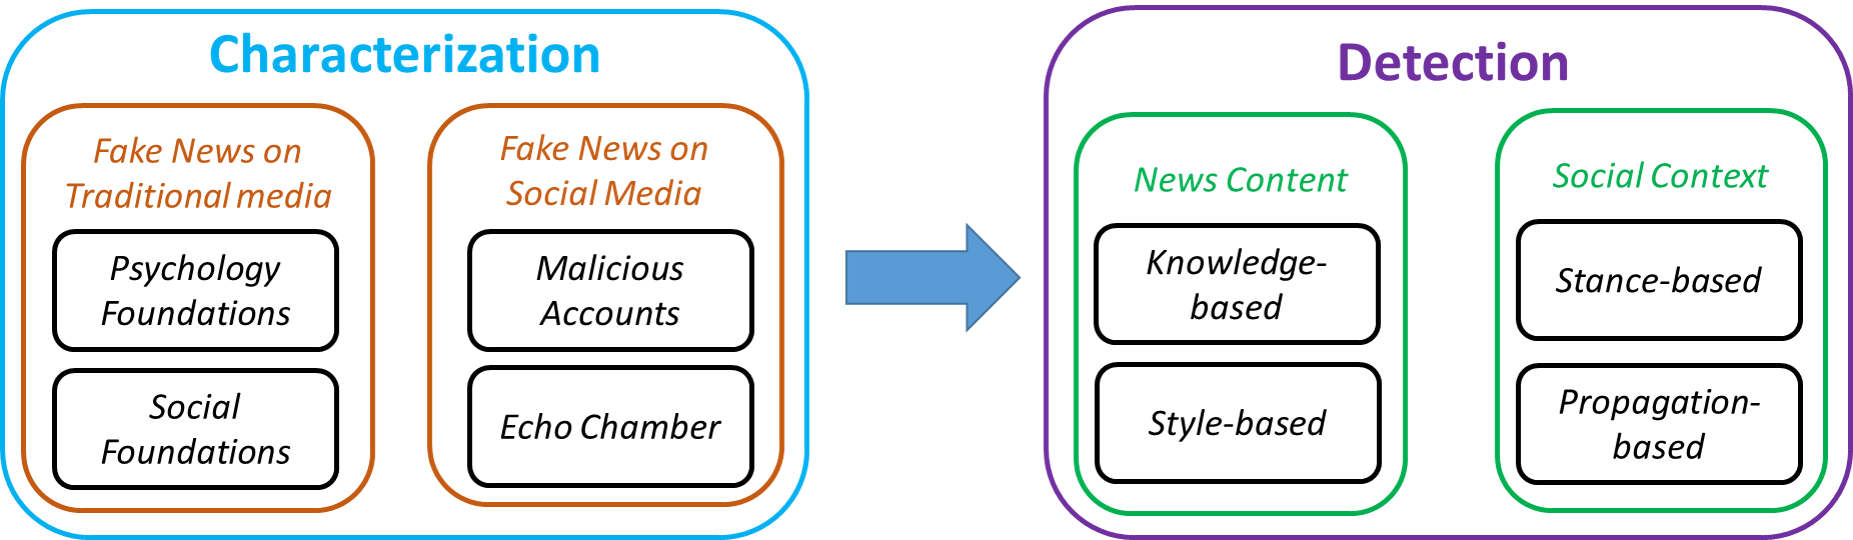
\includegraphics[height=3cm]{framework.png}
{\footnotesize \url{https://arxiv.org/abs/1708.01967} for details.}
\end{block}
\end{frame}

%-----------------------------------------------
\begin{frame}{}
\begin{block}{Future Directions}
\vspace{.4cm}
\centering
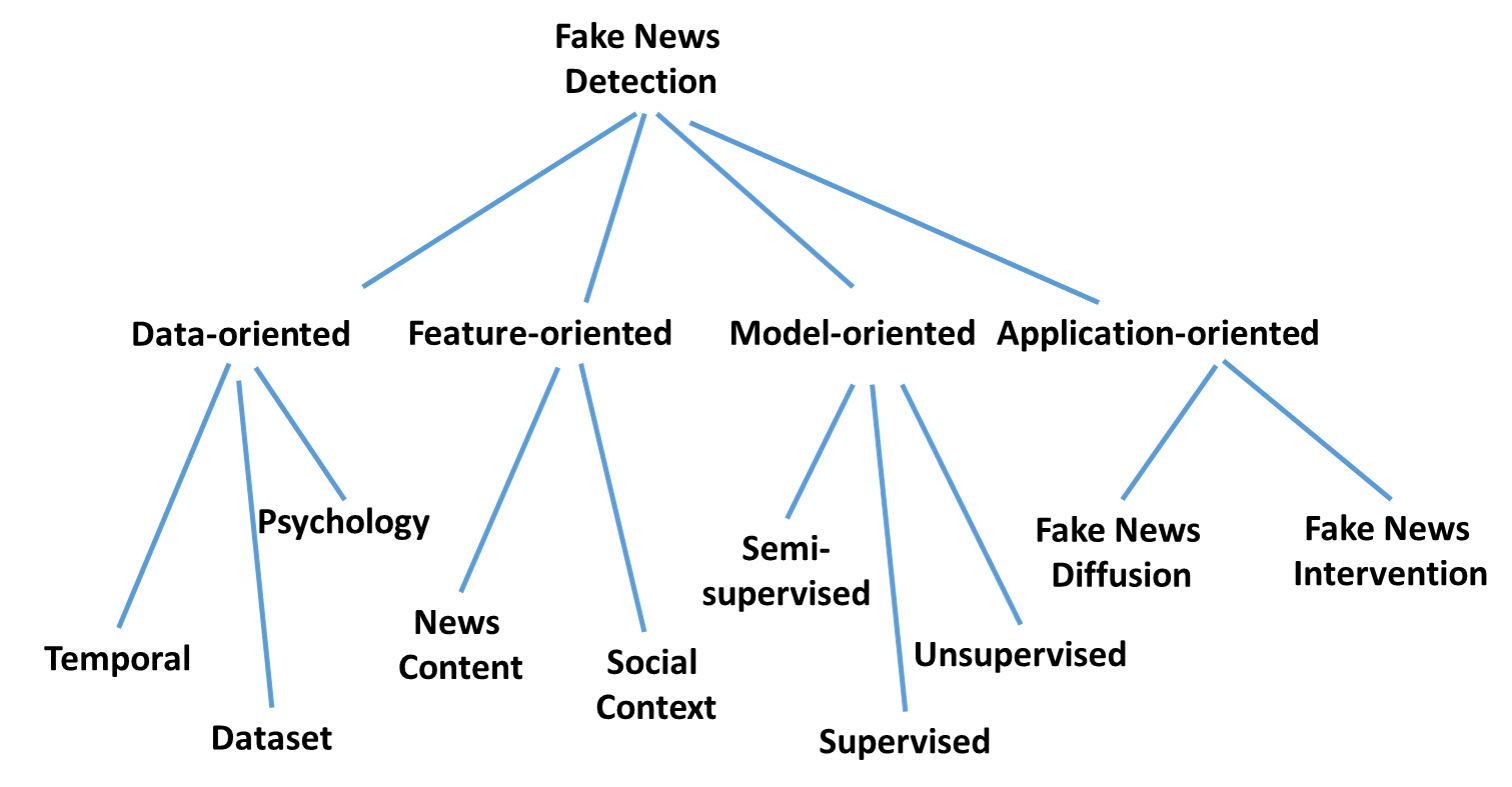
\includegraphics[height=5.5cm]{future_direction.png}
{\footnotesize \url{https://arxiv.org/abs/1708.01967} for details.}
\end{block}
\end{frame}

%-----------------------------------------------
\begin{frame}{Building a Bayesian Model for Events}
Before reading anything,\\we can use prior knowledge from historical data.
\vspace{0.8cm}
\begin{block}{Valid Probability Model}
A probability model must satisfy:
\pause
\begin{enumerate}
    \item Cover all possible events.
    \item Assign probabilities to each event.
    \item Probabilities sum to one.
\end{enumerate}
\end{block}
\end{frame}

{
\setbeamercolor{background canvas}{bg=green!10}
%-----------------------------------------------
\begin{frame}{We’re Using \texttt{R} Instead of Python}
\begin{block}{Python}
\begin{itemize}
\item "Can do everything" ... installs $n$ packages, breaks after update
\item Stack Overflow becomes your TA
\end{itemize}
\end{block}
\begin{block}{\texttt{R} \quad \rightarrow \quad \url{https://cran.r-project.org}}
\begin{itemize}
\item Literally for statistics; \hl{\texttt{lm(y \textasciitilde{} x)}} and \ul{move on} with your life
\item Excellent, open-source, keeps us focused on data analysis,\\... and I enjoy sleeping at night!
\end{itemize}
\end{block}
\mbox{\textbf{What I Need From You:} learn concepts, analyze data, pass the class!}\\
\textbf{What I Do Not Need:} a 2-hour debate about virtual environments.
\end{frame}
}

%-----------------------------------------------
\begin{frame}[fragile]{}

\begin{columns}[t]
\begin{column}{0.285\textwidth}
\begin{block}{Dataset}
\begin{minted}[fontsize=\footnotesize, linenos]{r}
# Load packages
library(bayesrules)
library(tidyverse)
library(janitor)

# Import article data
data(fake_news)

fake_news %>% 
  tabyl(type) %>% 
  adorn_totals("row")
#  type   n percent
#  fake  60     0.4
#  real  90     0.6
# Total 150     1.0
\end{minted}
\end{block}
\end{column}

\begin{column}{0.53\textwidth}
\begin{block}{Prior Probability Model}
\begin{itemize}
    \item 150 news articles:\\60 fake, 90 real
    \item $P(\text{Fake}) = \frac{60}{150} = 0.40$.\\
          Before looking at the headline, the prior probability that an article is fake is 40\%.
\end{itemize}
\end{block}
\end{column}
\end{columns}
\end{frame}

%-----------------------------------------------
\begin{frame}{}
\textbf{Prior Belief}: there is a 40\% chance an article is fake before observing any evidence.
\[
P(B)=0.40 \quad \leftrightarrow \quad P(B^c)=0.60
\]
where \(B\): article is \textbf{fake}, \(B^c\): article is \textbf{real}.
\vspace{0.2cm}
\[
P(B) + P(B^c) = 0.40 + 0.60 = 1
\]
\begin{center}
\begin{tabular}{c|ccc}
\textbf{Event} & \(B\) & \(B^c\) & Total \\
\hline
Probability & 0.4 & 0.6 & 1
\end{tabular}
\end{center}
\end{frame}

%-----------------------------------------------
\begin{frame}{}
\begin{block}{}
Bayesian reasoning to estimate whether a news article is fake:
\vspace{0.8em}

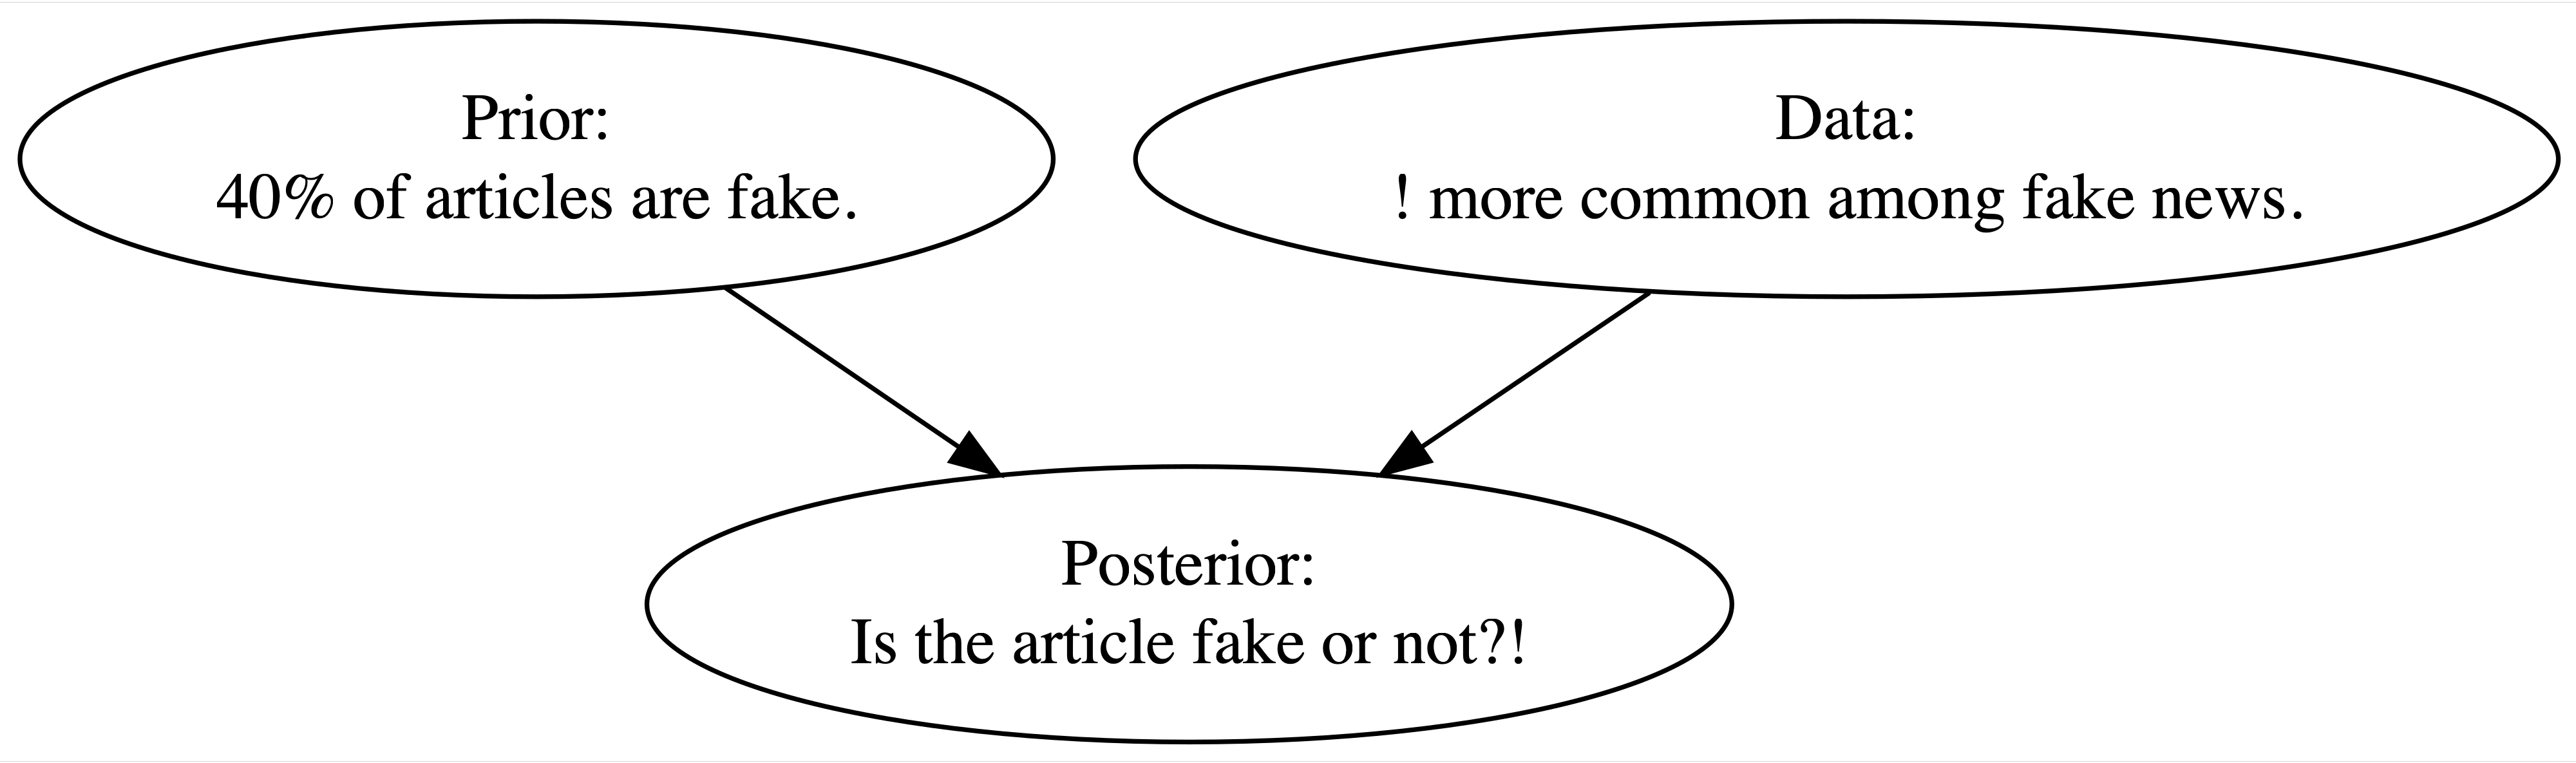
\includegraphics[height=3.3cm]{fake_news_diagram.png}
\end{block}
\end{frame}

%-----------------------------------------------
\begin{frame}{}
\begin{block}{DAG: Directed Acyclic Graph}
\begin{center}
\begin{tikzpicture}[
    node distance=3cm,
    every node/.style={circle, draw, thick, minimum size=1.3cm}
]
\node (A) {\(A\)};
\node[right of=A] (B) {\(B\)};
\draw[-Triangle, thick] (A) -- (B);
\end{tikzpicture}
$
A = \text{exclamation points "!"}
\quad
\quad
B = \text{fake status "\emoji{disguised-face}"}$
\end{center}
\begin{itemize}
    \item A \textbf{DAG} shows how variables are connected.
    \item The arrow means \(A\) may be associate with \(B\).
    \item \textbf{Acyclic} means the arrows do not loop back.
\end{itemize}
\end{block}
\end{frame}

%-----------------------------------------------
\begin{frame}{}
\begin{block}{DAGs and Conditional Probability}
\begin{itemize}
    \item The DAG suggests that the chance of \(B\) may depend on \(A\).
    \[
    P(B \mid A)
    \]
    \item[] In words: the probability of article is fake \textbf{given}\\
            \hspace{4cm}the exclamation point in the title.
    \pause
    \item If \(A\) changes the probability of \(B\),\\
          \hspace{2cm}then the events are \textbf{dependent}.
    \[
    P(B \mid A) \neq P(B)
    \]
    \item \pause If knowing \(A\) does not change the probability of \(B\),\\
          \hspace{5cm}then they are \textbf{independent}.
    \[
    P(B \mid A) = P(B)
    \]
\end{itemize}
\end{block}
\end{frame}

%-----------------------------------------------
\begin{frame}[fragile]{}
\begin{minted}[fontsize=\footnotesize, linenos]{r}
# Transposed version of head()
# ... makes possible to see all columns in a data frame
glimpse(fake_news)
\end{minted}

\vspace{1.em}

Observed headline pattern:

\begin{minted}[fontsize=\footnotesize, linenos]{r}
# Tabulate exclamation usage and article type
fake_news %>% 
  tabyl(title_has_excl, type) %>% 
  adorn_totals("row")
# title_has_excl fake real
#          FALSE   44   88
#           TRUE   16    2
#          Total   60   90
\end{minted}
\end{frame}

%-----------------------------------------------
\begin{frame}{}
\begin{block}{Exclamation Points as Evidence}
\vspace{0.4em}
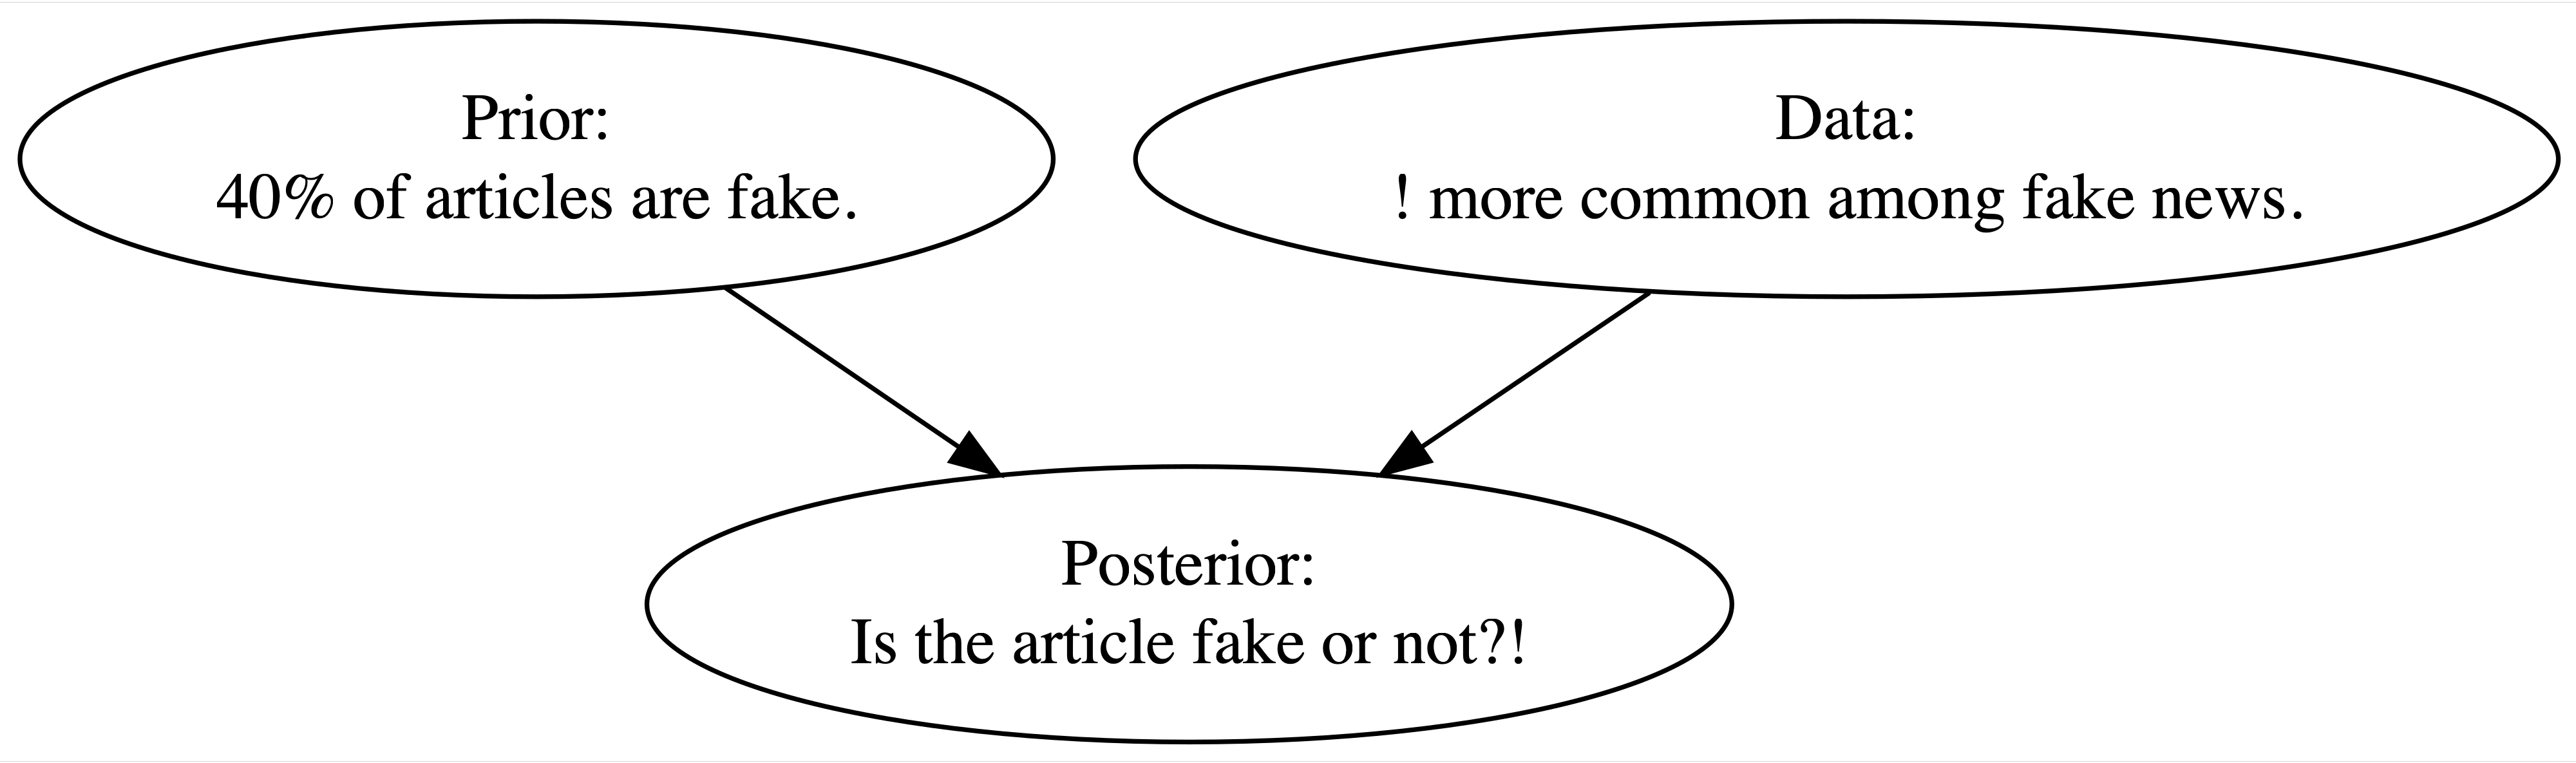
\includegraphics[height=3.4cm]{fake_news_diagram.png}
\begin{table}
\centering
\begin{tabular}{lrrr}
\toprule
\textbf{Title Has ``!''} & \textbf{Fake} & \textbf{Real} & \textbf{Total} \\
\midrule
Yes & 16 & 2  & 18 \\
No  & 44 & 88 & 132 \\
\midrule
Total & 60 & 90 & 150 \\
\bottomrule
\end{tabular}
\end{table}
\end{block}
\end{frame}

%-----------------------------------------------
\begin{frame}{}
\begin{block}{Conditional Probability \& Likelihood}
\begin{table}
\centering
\begin{tabular}{lrrr}
\toprule
\textbf{Title Has ``!''} & \textbf{Fake} & \textbf{Real} & \textbf{Total} \\
\midrule
Yes & 16 & 2  & 18 \\
No  & 44 & 88 & 132 \\
\midrule
Total & 60 & 90 & 150 \\
\bottomrule
\end{tabular}
\end{table}
\begin{center}
$P(! \mid \text{Fake}) = \frac{16}{60} \approx 0.267$,
$P(! \mid \text{Real}) = \frac{2}{90} \approx 0.022$
\end{center}
\vspace{0.4em}
An exclamation point increases the probability that an article \hl{is fake}.
\end{block}
\end{frame}

%-----------------------------------------------
\begin{frame}{}
\begin{block}{Conditional Probability \& Likelihood}
\[
\begin{aligned}
B &: \text{article is fake} \\
B^c &: \text{article is real}
\end{aligned}
\]
\[
\begin{aligned}
A &: \text{article uses exclamation points} \\
A^c &: \text{article does not use exclamation points}
\end{aligned}
\]
From the data:
\[
P(A \mid B)=0.267 \qquad P(A \mid B^c)=0.022
\]
Fake news articles are \textbf{much more likely} to use exclamation points than real news articles.
\end{block}
\end{frame}


%-----------------------------------------------
\begin{frame}{}
\begin{block}{Conditional vs Unconditional Probability}
\begin{itemize}
    \item \textbf{Unconditional probability} is the chance something happens without extra information.
    \[
    P(A)
    \]
    \item \textbf{Conditional probability} is the chance something happens given that something else is already known.
    \[
    P(A \mid B)
    \]
    \item Comparing \(P(A)\) and \(P(A \mid B)\) tells us whether knowing \(B\) changes how likely \(A\) is.
\end{itemize}
\end{block}
\end{frame}

%-----------------------------------------------
\begin{frame}{}
\begin{block}{Independent Events}
\begin{itemize}
    \item Two events are \textbf{independent} if knowing one happens does not change the probability of the other.
    \item \textcolor{aggiemaroon!70}{\emph{Example}: rolling a die and flipping a coin are independent, because the die result \textbf{does not} affect the coin flip.}
    \item In symbols:
    \[
    P(A \mid B) = P(A)
    \]
\end{itemize}
\end{block}
\end{frame}

%-----------------------------------------------
\begin{frame}{}
\begin{block}{From Probability to Likelihood}
\begin{itemize}
    \item Earlier, we computed:
    \[
    P(A \mid B)=0.2667
    \qquad
    P(A \mid B^c)=0.0222
    \]
    \item Fake articles are much more likely to use exclamation points.
    \item Suppose we already observed an article with exclamations.
    \item[] Now the question becomes:\\
          \centering \textit{Is the article more likely fake or real?}
\end{itemize}
\end{block}
\end{frame}

%-----------------------------------------------
\begin{frame}{}
\begin{block}{What is Likelihood?}
\begin{itemize}
    \item \textbf{Probability} starts with a known cause and predicts data.
    \[
    P(A \mid B)
    \]
    \item \textbf{Likelihood} starts with observed data and compares possible causes.
    \[
    \mathcal{L}(B \mid A)=P(A \mid B)
    \]
    \item In our example:
    \begin{itemize}
        \item \(A\): article uses exclamation points
        \item \(B\): article is fake
        \item Since
              \[
              P(A \mid B) > P(A \mid B^c)
              \]
              \emph{exclamation} provide evidence that the article may be fake.
        \end{itemize}
\end{itemize}
\end{block}
\end{frame}

%-----------------------------------------------
\begin{frame}{}
\begin{center}
\begin{tabular}{p{4cm}|p{4cm}}
\textbf{Probability} & \textbf{Likelihood} \\
\hline
Known condition & Known data \\
Predicts outcomes & Compares explanations \\
\[
P(A \mid B)
\]
& 
\[
\mathcal{L}(B \mid A)
\]
\end{tabular}
\end{center}
\begin{itemize}
\item The distinction is \textbf{subtle}, especially since people use the terms “likelihood” and “probability” interchangeably in casual conversation.
\item Likelihood \textbf{helps us decide} which explanation best fits the observed data.
\end{itemize}
\end{frame}

%-----------------------------------------------
\begin{frame}{}
\begin{block}{}
\begin{itemize}
\item The likelihood function \textbf{is not} a probability function, but rather provides a framework to compare the relative compatibility of our exclamation point data with $B$ and $B^c$.
\end{itemize}
\begin{table}[h]
\centering
\begin{tabular}{lccc}
\hline
\textbf{Event}              & \(B\)  & \(B^c\) & \textbf{Total} \\
\hline
Prior probability           & 0.4    & 0.6     & 1              \\[0.1cm]
Likelihood $(\cdot \mid A)$ & 0.2667 & 0.0232  & \hl{0.2889}    \\
\hline
\end{tabular}
\end{table}
\end{block}
\end{frame}

{
\setbeamercolor{background canvas}{bg=blue!10}
%-----------------------------------------------
\begin{frame}{}
\begin{block}{Quiz}
Two boxes are available:

\begin{itemize}
    \item Box 1 contains 4 red and 2 green balls.
    \item Box 2 contains 2 red and 4 green balls.
    \item The probability of choosing either box is equal:
    \[
    P(E_1)=P(E_2)=\frac12.
    \]
    \item A box is selected at random, and one ball is drawn.
    \item Study the \textbf{likelihood} of observing a red ball under each box.
\end{itemize}
\end{block}
\end{frame}

%-----------------------------------------------
\begin{frame}{}
\begin{block}{}
\begin{center}
\begin{tikzpicture}[scale=1]

    % Outer rectangle
    \draw[thick] (0,0) rectangle (10,5);

    % Divider
    \draw[thick] (5.,0) -- (5.,5);

    % Labels
    % \node at (2.3,5.4) {$B1$};
    % \node at (7.7,5.4) {$B2$};

    % Left side label
    \node at (0.8,4.2) {$B_1$};

    % Right side label
    \node at (9.2,4.2) {$B_2$};

    % Red ellipse
    \draw[red, thick] (4.75,2.5) ellipse (3.2 and 1.2);
    \node[red] at (6.9,2.0) {$R$};

    % Left box red balls
    \fill[red] (2.7,3.0) circle (0.12);
    \fill[red] (3.8,3.0) circle (0.12);
    \fill[red] (2.1,2.2) circle (0.12);
    \fill[red] (3.3,1.7) circle (0.12);

    % Left box green balls
    \fill[green!70!black] (1.4,3.8) circle (0.12);
    \fill[green!70!black] (0.7,2.5) circle (0.12);

    % Right box red balls
    \fill[red] (6.5,2.7) circle (0.12);
    \fill[red] (5.9,1.8) circle (0.12);

    % Right box green balls
    \fill[green!70!black] (7.4,3.9) circle (0.12);
    \fill[green!70!black] (8.8,3.2) circle (0.12);
    \fill[green!70!black] (8.9,1.5) circle (0.12);
    \fill[green!70!black] (6.7,0.9) circle (0.12);

\end{tikzpicture}
\end{center}
\end{block}
\end{frame}

%-----------------------------------------------
\begin{frame}{}
\begin{block}{}
\small
\textbf{Answer:}
{\color{blue}
A red ball is more consistent with Box 1 than with Box 2.\\[.1cm]

The likelihoods are:
$P(R\mid B_1)=\frac46=\frac23$
and
$P(R\mid B_2)=\frac26=\frac13.$\\[.1cm]

So, if Box 1 had been selected, observing a red ball would be more likely.

\begin{center}
$P(R\mid B_1) > P(R\mid B_2)$
\end{center}

Therefore, the red ball provides stronger evidence for Box 1 than for Box 2.
\[
\frac{P(R\mid B_1)}{P(R\mid B_2)} = \frac{\frac23}{\frac13} = 2
\]
The observed red ball is \textbf{twice} as likely under Box 1 as under Box 2. Since the boxes were equally likely before the draw, the red ball favors Box 1.
}
\end{block}
\end{frame}
}

%-----------------------------------------------
\begin{frame}{}
\begin{block}{Recap}
\[
\begin{aligned}
&A   = \text{article uses exclamation points}\\
&A^c = \text{article does not use exclamation points}\\
&B    = \text{article is fake news}\\
&B^c  = \text{article is real news}
\end{aligned}
\]
\vspace{0.2cm}

From the prior model:
\[
P(B)=0.4
\qquad
P(B^c)=0.6
\]

So, 40\% of articles are fake and 60\% are real.
\end{block}
\end{frame}

%-----------------------------------------------
\begin{frame}{}
\begin{block}{Normalizing Constants}
\begin{itemize}
    \item The marginal probability of observing exclamation points across all articles is $P(A)$.
    \item This is called the \textbf{normalizing constant}.
    \pause
    \item To calculate it, we split articles into two groups:\\
          \hspace{2cm}$P(A)=P(A \cap B)+P(A \cap B^c)$
    \item That is:\\ \mbox{$\text{Exclamations} = \text{fake with exclamations} + \text{real with exclamations}$}
\end{itemize}
\end{block}
\end{frame}

%-----------------------------------------------
\begin{frame}{}
\begin{block}{Joint Probability Table}
\[
\begin{array}{c|ccc}
 & B & B^c & \text{Total} \\
\hline
A & P(A \cap B) & P(A \cap B^c) & P(A) \\
A^c & P(A^c \cap B) & P(A^c \cap B^c) & P(A^c) \\
\hline
\text{Total} & 0.4 & 0.6 & 1
\end{array}
\]
\vspace{0.2cm}
\begin{itemize}
    \item Each inside cell is a \textbf{joint probability}.
    \item For example: $P(A \cap B)$ means the probability that an article is fake and uses exclamation points.
\end{itemize}
\end{block}
\end{frame}

%-----------------------------------------------
\begin{frame}{}
\begin{block}{Fake Articles \textbf{with} Exclamation Points}
\begin{itemize}
    \item To determine the probabilities of these joint events, note that 40\% of articles are fake and 26.67\% of fake articles use exclamation points, $P(B) = 0.4$ and $P(A \mid B) = 0.2667$. 
    \item The joint probability is
    $P(A \cap B) = P(A \mid B) ~ P(B) = 0.2667 \cdot 0.4 = 0.1067$
    \item So, 10.67\% of all articles are fake and use exclamation points.
\end{itemize}
\end{block}
\end{frame}

%-----------------------------------------------
\begin{frame}{}
\begin{block}{}
\[
\begin{array}{c|ccc}
 & B & B^c & \text{Total} \\
\hline
A & $0.4 \cdot 16/60 = \textbf{0.107}$ & P(A \cap B^c) & $32/150 = 0.12$ \\
A^c & P(A^c \cap B) & P(A^c \cap B^c) & $118/150 = 0.78$ \\
\hline
\text{Total} & \textbf{0.4} & 0.6 & 1
\end{array}
\]
\end{block}
\end{frame}

%-----------------------------------------------
\begin{frame}{}
\begin{block}{Fake Articles \textbf{without} Exclamation Points}
\begin{itemize}
    \item Since 26.67\% of fake articles use exclamation points, $1 - 0.2667 = 73.33\%$ do not use exclamation points.
    \item Then, $P(A^c \cap B) = P(A^c\mid B)~P(B) = 0.7333 \cdot 0.4 = 0.2933$
    \item So, 29.33\% of all articles are fake and do not use exclamation.
\end{itemize}
\end{block}
\end{frame}

%-----------------------------------------------
\begin{frame}{}
\begin{block}{Checking the Fake Article Total}
The fake-news column is split into two parts:

\[P(A \cap B) \quad \text{and} \quad P(A^c \cap B)\]

Therefore,
\[
P(B)=P(A \cap B)+P(A^c \cap B)
\]
\[
P(B)=0.1067+0.2933
\]
\[
P(B)=0.4
\]

This matches the prior probability that an article is fake.
\end{block}
\end{frame}

%-----------------------------------------------
\begin{frame}{}
\begin{block}{Real Articles}
From the likelihood function: $P(A\mid B^c)=0.0222$\\

So only 2.22\% of real articles use exclamation points.\\

The joint probability is
\[
P(A \cap B^c)=P(A\mid B^c)P(B^c)
\]
\[
P(A \cap B^c)=0.0222 \cdot 0.6
\]
\[
P(A \cap B^c)=0.0133
\]

So, 1.33\% of all articles are real and use exclamation points.
\end{block}
\end{frame}

%-----------------------------------------------
\begin{frame}{}
\begin{block}{Real Articles without Exclamation Points}
Since
\[
P(A\mid B^c)=0.0222
\]
we have
\[
P(A^c\mid B^c)=1-0.0222
\]
\[
P(A^c\mid B^c)=0.9778
\]

Then
\[
P(A^c \cap B^c)=P(A^c\mid B^c) ~ P(B^c)
\]
\[
P(A^c \cap B^c)=0.9778 \cdot 0.6
\]
\[
P(A^c \cap B^c)=0.5867
\]
\end{block}
\end{frame}

%-----------------------------------------------
\begin{frame}{}
\begin{block}{Completed Joint Probability Table}
\[
\begin{array}{c|ccc}
 & B & B^c & \text{Total} \\
\hline
A   & 0.107 & 0.013 & 0.12 \\
A^c & 0.293 & 0.587 & 0.88 \\
\hline
\text{Total} & 0.4 & 0.6 & 1
\end{array}
\]

The row total for \(A\) gives the \textbf{normalizing constant}:
\[
P(A) = 0.107 + 0.013 = \boxed{0.12}
\]

So, 12\% of all articles use exclamation points.
\end{block}
\end{frame}

%-----------------------------------------------
\begin{frame}{}
\begin{block}{Joint Probability}
The calculations use the relationship
\[
P(A \cap B)=P(A\mid B)P(B)
\]

This connects: $~ \text{joint probability}$\\

with: $~ \text{conditional probability} \times \text{prior probability}$\\

Rearranging gives the conditional probability formula:
\[
P(A\mid B)=\frac{P(A \cap B)}{P(B)}
\]

\textcolor{aggiemaroon!70}{
PS. If \(A\) and \(B\) are \textbf{independent}, then:
$P(A \cap B) = P(A) ~ P(B)$
}
\end{block}
\end{frame}


%-----------------------------------------------
\begin{frame}{}
\begin{block}{
Representation of Conditional Probability
}
\begin{figure}[h]
\centering
\[
P(A\mid B)
=
\frac{P(A\cap B)}{P(B)}=
\frac{
\begin{tikzpicture}[baseline=-0.5ex,scale=0.8]
    % Rectangle
    \draw (0,0) rectangle (4,2);

    % Circles
    \begin{scope}
        \clip (1.2,1) circle (0.8);
        \fill[AggieMaroon!35] (2.4,1) circle (0.8);
    \end{scope}

    \draw (1.2,1) circle (0.8);
    \draw (2.4,1) circle (0.8);

    \node at (0.75,1) {$A$};
    \node at (2.8,1) {$B$};
\end{tikzpicture}
}
{
\begin{tikzpicture}[baseline=-0.5ex,scale=0.8]
    % Rectangle
    \draw (0,0) rectangle (4,2);

    % Event B
    \fill[AggieMaroon!35] (2.4,1) circle (0.8);

    \draw (1.2,1) circle (0.8);
    \draw (2.4,1) circle (0.8);

    \node at (0.75,1) {$A$};
    \node at (2.8,1) {$B$};
\end{tikzpicture}
}
\]
\end{figure}
\end{block}
\end{frame}

%-----------------------------------------------
\begin{frame}{}
\begin{block}{Conditional Probability}
Conditional probability answers the question:
\[
\textit{“What is the probability of } A \textit{ given that } B \textit{ has occurred?”}
\]

The definition is:
\[
P(A \mid B) = \frac{P(A \cap B)}{P(B)}
\qquad \text{where } P(B) \neq 0
\]

\begin{itemize}
    \item Start with the probability that both \(A\) and \(B\) occur
    \item Restrict attention only to situations where \(B\) occurs
    \item Measure how often \(A\) also occurs
\end{itemize}
\vspace{0.4cm}

\textcolor{aggiemaroon!70}{
\textbf{Example:}
$
P(\text{Rain} \mid \text{Cloudy})
=
\frac{
P(\text{Rain and Cloudy})
}{
P(\text{Cloudy})
}
$
}
\end{block}
\end{frame}

%-----------------------------------------------
\begin{frame}{}
\begin{block}{Law of Total Probability}
Suppose event \(A\) can happen in two distinct ways:
\[
A \cap B
\qquad \text{or} \qquad
A \cap B^c
\]

Since \(B\) and \(B^c\) cover all possibilities, we can write:
\[
P(A) = P(A \cap B) + P(A \cap B^c)
\]

Using the joint probability rule:
\[
P(A \cap B) = P(A \mid B)P(B)
\]

we get the \textbf{Law of Total Probability}:
\[
P(A)
=
P(A \mid B)P(B)
+
P(A \mid B^c)P(B^c)
\]
\end{block}
\end{frame}

%-----------------------------------------------
\begin{frame}{}
\begin{block}{Exclamation Points in News Articles}
\[
\begin{aligned}
A &= \text{article uses an exclamation point}\\
B &= \text{article is fake news}
\end{aligned}
\]

\[
P(A \mid B)=0.2667,
\qquad
P(B)=0.4
\]
\[
P(A \mid B^c)=0.0222,
\qquad
P(B^c)=0.6
\]
Then:
\[
P(A)
=
0.2667~(0.4) + 0.0222~(0.6)
\]
\[
P(A)
=
0.1067 + 0.0133
=
0.12
\]\\
So, about \textbf{12\% of all articles} use exclamation points.
\end{block}
\end{frame}

%-----------------------------------------------
\begin{frame}{}
\begin{block}{}
\[
\begin{array}{c|ccc}
 & B & B^c & \text{Total} \\
\hline
A   & 0.107 & 0.013 & 0.12 \\
A^c & 0.293 & 0.587 & 0.88 \\
\hline
\text{Total} & 0.4 & 0.6 & 1
\end{array}
\]

\[
P(A) = 0.107 + 0.013 = \boxed{0.12}
\]

\end{block}
\end{frame}

%-----------------------------------------------
\begin{frame}{}
\begin{block}{Posterior probability model via Bayes’ rule}
What is the probability that the latest article is fake, given that it uses an exclamation point?
\end{block}

%\begin{block}{Posterior probability}
%\[
%P(B\mid A)
%\]
%
%\begin{itemize}
%    \item $B$: the article is fake.
%    \item $A$: the article uses an exclamation point.
%    \item Goal: update the probability of $B$ after observing $A$.
%\end{itemize}
%
%
%\end{block}
\end{frame}

%------------------------------------------------
% Slide 2
%------------------------------------------------
%\begin{frame}{Intuition from the News Example}
%
%\begin{columns}[T,onlytextwidth]
%
%\column{0.52\textwidth}
%
%\begin{itemize}
%    \item Among all articles, 12\% use exclamation points.
%
%    \item Within that 12\%, the proportions are:
%    \begin{itemize}
%        \item 88.9\% fake news.
%        \item 11.1\% real news.
%    \end{itemize}
%
%    \item Therefore, after seeing an exclamation point,
%    the posterior probability that the article is fake is 88.9\%.
%\end{itemize}
%
%\column{0.43\textwidth}
%
%\begin{block}{Interpretation}
%\[
%P(B\mid A)=0.889
%\]
%
%\small
%The exclamation point is evidence because it is more common
%among fake articles than real articles.
%\end{block}
%
%\end{columns}
%
%\end{frame}

%------------------------------------------------
% Slide 3
%------------------------------------------------
%\begin{frame}{Bayes' Rule for Events}
%
%\begin{block}{Posterior probability of $B$ given $A$}
%
%For events $A$ and $B$, Bayes' Rule combines a prior probability
%with a likelihood:
%
%\[
%P(B\mid A)
%=
%\frac{P(A\cap B)}{P(A)}
%=
%\frac{P(B)L(B\mid A)}{P(A)}.
%\]
%
%\end{block}
%
%\vspace{0.25cm}
%
%The normalizing constant is found using the Law of Total Probability:
%
%\[
%P(A)
%=
%P(B)L(B\mid A)
%+
%P(B^c)L(B^c\mid A).
%\]
%
%\vspace{0.25cm}
%
%\begin{center}
%\Large
%\[
%\text{posterior}
%=
%\frac{\text{prior}\cdot\text{likelihood}}
%     {\text{normalizing constant}}
%\]
%\end{center}
%
%\end{frame}

%------------------------------------------------
% Slide 4
%------------------------------------------------
%\begin{frame}{Applying Bayes' Rule to the Article}
%
%\begin{block}{Calculation}
%
%\[
%P(B\mid A)
%=
%\frac{P(B)L(B\mid A)}{P(A)}
%=
%\frac{0.4\cdot 0.2667}{0.12}
%=
%0.889.
%\]
%
%\end{block}
%
%\vspace{0.25cm}
%
%\begin{center}
%
%\begin{tabular}{lccc}
%\hline
%\textbf{Event} & $B$ & $B^c$ & \textbf{Total} \\
%\hline
%Prior probability     & 0.400 & 0.600 & 1 \\
%Posterior probability & 0.889 & 0.111 & 1 \\
%\hline
%\end{tabular}
%
%\end{center}
%
%\vspace{0.25cm}
%
%\begin{itemize}
%    \item Prior belief: 40\% chance the incoming article is fake.
%    \item Observation: the title contains an exclamation point.
%    \item Updated belief: the chance the article is fake rises to 88.9\%.
%\end{itemize}
%
%\end{frame}

%-----------------------------------------------
\begin{frame}{}
\begin{block}{}

\end{block}
\end{frame}

%-----------------------------------------------
\begin{frame}{}
\begin{block}{}

\end{block}
\end{frame}

%-----------------------------------------------
\begin{frame}{}
\begin{block}{}

\end{block}
\end{frame}

%-----------------------------------------------
\begin{frame}{}
\begin{block}{}

\end{block}
\end{frame}

%-----------------------------------------------
\begin{frame}{}
\begin{block}{}
\[
P(\text{Fake} \mid !) =
\frac{P(\text{Fake}) ~ P(! \mid \text{Fake})}{P(!)}
\]
\end{block}
\end{frame}

%-----------------------------------------------
\begin{frame}{}
\begin{block}{}

\end{block}
\end{frame}


















%-----------------------------------------------
\begin{frame}{}
\begin{block}{Calculating Joint and Conditional Probabilities}
\begin{itemize}
\item 
\item 
\item 
\end{itemize}
\end{block}
\end{frame}

%-----------------------------------------------
\begin{frame}{}
\begin{block}{Posterior Probability Model via Bayes’ Rule}
\begin{itemize}
\item 
\item 
\item 
\end{itemize}
\end{block}
\end{frame}

%-----------------------------------------------
\begin{frame}{}
\begin{block}{Posterior Simulation}
\begin{itemize}
\item 
\item 
\item 
\end{itemize}
\end{block}
\end{frame}

%-----------------------------------------------
\begin{frame}{Building a Bayesian Model for Random Variables}
\begin{block}{Prior Probability Model}
\begin{itemize}
\item 
\item 
\item 
\end{itemize}
\end{block}
\end{frame}

%-----------------------------------------------
\begin{frame}{}
\begin{block}{Discrete Probability Model}
\begin{itemize}
\item 
\item 
\item 
\end{itemize}
\end{block}
\end{frame}

%-----------------------------------------------
\begin{frame}{}
\begin{block}{The Binomial Data Model}
\begin{itemize}
\item 
\item 
\item 
\end{itemize}
\end{block}
\end{frame}

%-----------------------------------------------
\begin{frame}{}
\begin{block}{Conditional Probability Model of Data $Y$}
\begin{itemize}
\item 
\item 
\item 
\end{itemize}
\end{block}
\end{frame}

%-----------------------------------------------
\begin{frame}{}
\begin{block}{The Binomial Model}
\begin{itemize}
\item 
\item 
\item 
\end{itemize}
\end{block}
\end{frame}

%-----------------------------------------------
\begin{frame}{}
\begin{block}{The Binomial Likelihood Function}
\begin{itemize}
\item 
\item 
\item 
\end{itemize}
\end{block}
\end{frame}

%-----------------------------------------------
\begin{frame}{}
\begin{block}{Probability Mass Functions vs Likelihood Functions}
\begin{itemize}
\item 
\item 
\item 
\end{itemize}
\end{block}
\end{frame}

%-----------------------------------------------
\begin{frame}{}
\begin{block}{Normalizing Constant}
\begin{itemize}
\item 
\item 
\item 
\end{itemize}
\end{block}
\end{frame}

%-----------------------------------------------
\begin{frame}{}
\begin{block}{Posterior Probability Model}
\begin{itemize}
\item 
\item 
\item 
\end{itemize}
\end{block}
\end{frame}

%-----------------------------------------------
\begin{frame}{}
\begin{block}{Bayes’ Rule for Variables}
\begin{itemize}
\item 
\item 
\item 
\end{itemize}
\end{block}
\end{frame}

%-----------------------------------------------
\begin{frame}{}
\begin{block}{Posterior Shortcut}
\begin{itemize}
\item 
\item 
\item 
\end{itemize}
\end{block}
\end{frame}

%-----------------------------------------------
\begin{frame}{}
\begin{block}{Proportionality}
\begin{itemize}
\item 
\item 
\item 
\end{itemize}
\end{block}
\end{frame}

%-----------------------------------------------
\begin{frame}{}
\begin{block}{Posterior Simulation}
\begin{itemize}
\item 
\item 
\item 
\end{itemize}
\end{block}
\end{frame}

{
\setbeamercolor{background canvas}{bg=blue!10}
%-----------------------------------------------
\begin{frame}{}
\begin{block}{Quiz 1}
A medical test correctly detects a disease 95\% of the time when the disease is present.
This value represents:
\begin{itemize}
\item[a.] Prior probability
\item[b.] Posterior probability
\item[c.] False positive rate
\item[d.] Likelihood
\end{itemize}
\end{block}
\end{frame}

%-----------------------------------------------
\begin{frame}{}
\textbf{Answer:}
{\color{blue}
d. Likelihood\\

The statement describes: $P(\text{Test positive} \mid \text{Disease present}) = 0.95$\\

This is the probability of observing the test result given that the disease is present, 
which represents the \ul{likelihood} (also called \textbf{sensitivity} or \textbf{true positive rate}).\\

- \textbf{Prior}: Probability of disease before observing the test result.\\
- \textbf{Posterior}: Probability of disease after observing the test result.\\
- \textbf{False positive rate}: Probability that the test is positive when the disease is absent.
}
\end{frame}

%-----------------------------------------------
\begin{frame}{}
\begin{block}{Quiz 2}
A university uses an AI system to detect plagiarism.
\begin{itemize}
\item 5\% of assignments are actually plagiarized.
\item The AI flags plagiarized assignments 92\% of the time.
\item The AI incorrectly flags honest assignments 8\% of the time.
\end{itemize}
If an assignment is flagged, what is the probability it was actually plagiarized?
Briefly discuss whether the AI system seems reliable.
\end{block}
\end{frame}

%-----------------------------------------------
\begin{frame}{}
\begin{block}{}
\vspace{0.2cm}
\textbf{Answer:}
{\color{blue}
\[
\begin{aligned}
P(P\mid F)
=\frac{0.92\cdot 0.05}
       {0.92\cdot 0.05 + 0.08\cdot 0.95} \approx 0.377
\end{aligned}
\]

\vspace{0.2cm}
Approximately 37.7\% chance that it is actually plagiarism.\\
The system catches most plagiarism cases, but because plagiarism is rare, many flagged assignments are false positives.
}
\end{block}
\end{frame}

%-----------------------------------------------
\begin{frame}{}
\begin{block}{Quiz 3}
\begin{columns}[c]
% Left column: image
    \begin{column}{0.32\textwidth}
    \centering
    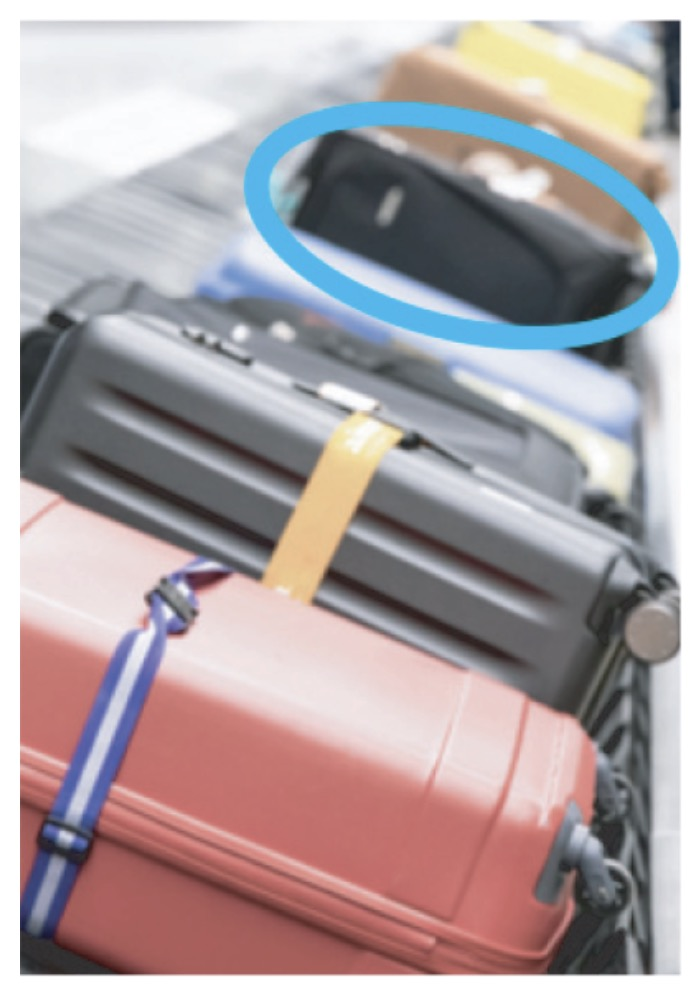
\includegraphics[width=3.75cm]{Bags.jpg}
    \end{column}
% Right column: text
    \begin{column}{0.66\textwidth}
    \small
    Let's suppose that you are an air traveler along with 99 other passengers from your flight, each of whom, like you, checked one item of luggage.
    
    \vspace{0.2cm}
    
    A recording piped through the speakers reminds you that:
    \emph{``Many bags look alike. Please check your bag carefully before exiting the terminal.''}
    
    \vspace{0.2cm}
    
    Indeed, your bag is one of the most popular models on the market, a medium-sized black rectangular case \textbf{used by 5\% of all travelers}.
    
    \vspace{0.2cm}
    
    Given your distance from the luggage chute, you can discern only the shape, size, and color of the bags that emerge, not any detailed markings on the bags.
    \end{column}
\end{columns}
\end{block}
\end{frame}

%-----------------------------------------------
\begin{frame}{}
\begin{block}{Quiz 3, cont.}
\begin{itemize}
\item[a.] Let's suppose that the \textbf{first bag} from your flight to enter the luggage carousel indeed has the same shape, size, and color as yours.
          Is it yours? Explain (i.e., calculate the posterior probability that the 1st bag is yours).

\vspace{0.4cm}
    
\item[b.] Now suppose that we continue to wait for our bag to appear, failing to see it among the first 98 bags to enter the carousel (i.e., only 2 bags are left to come off the airplane).
          Calculate the posterior probability that the \textbf{99th} bag, which also matches ours in shape, size, and color, is our own.
\end{itemize}
\end{block}
\end{frame}

%-----------------------------------------------
\begin{frame}{}
\textbf{Answer: a.}
{\color{blue}
\footnotesize
Let \(Y\) = first bag is yours, and \(M\) = first bag matches.

\[
\begin{aligned}
&P(Y)=\frac{1}{100}\\
&\mathcal{L}(Y^c\mid M)=P(M\mid Y^c)=0.05\\
&\mathcal{L}(Y\mid M)=P(M\mid Y)=1\\
\end{aligned}
\]

\[
\begin{aligned}
P(Y\mid M)&=\frac{P(M\mid Y)P(Y)}{P(M)}
          =\frac{P(M\mid Y)P(Y)}
                 {P(M\mid Y)P(Y)+P(M\mid Y^c)P(Y^c)}=\\
&=\frac{1\cdot 0.01}{1\cdot 0.01+0.05\cdot 0.99}
=\frac{0.01}{0.0595}\approx 0.168
\end{aligned}
\]

So even though the first bag matches, it is probably not yours.
}
\end{frame}

%-----------------------------------------------
\begin{frame}{}
\textbf{Answer: b.}
{\color{blue}
\footnotesize
\[
\begin{aligned}
P(Y\mid M)
&=\frac{1\cdot \tfrac{1}{\text{total of bags remaining}}}
       {1\cdot \tfrac{1}{\text{total of bags remaining}} + 0.05\cdot \tfrac{\text{total of bags remaining} - 1}{\text{total of bags remaining}}}\\
&\text{(if 2 bags remain)}\\
&=\frac{1\cdot \tfrac{1}{2}}
       {1\cdot \tfrac{1}{2} + 0.05\cdot \tfrac{1}{2}}=\frac{1}{1+0.05} \approx 0.9524
\end{aligned}
\]

There is a 95\% chance that the 99th bag is yours, given that it looks like yours.\\
Or, \hl{it is \textbf{19 times more likely} to be yours than not yours $^{(0.95/0.05 = 19)}$.}
}
\end{frame}
}

{
\setbeamercolor{background canvas}{bg=orange!10}
%-----------------------------------------------
\begin{frame}{Homework}
\begin{itemize}
\color{aggiemaroon}{
\item Submit your answers before the next class.
\item You may discuss with peers but submissions must be individual.
\item Responses may be shared anonymously during class discussion!
}
\end{itemize}
\end{frame}

%-----------------------------------------------
\begin{frame}{}
\begin{block}{Question 1}
Define the following events for a resident of a fictional town as:
\begin{itemize}
\item $A =$ drives 10 miles per hour above the speed limit,  
\item $B =$ gets a speeding ticket,  
\item $C =$ took statistics at the local college,  
\item $D =$ has used R,  
\item $E =$ likes the music of Prince, and  
\item $F =$ is a Texan.
\end{itemize}
Several facts about these events are listed next.
\end{block}
\end{frame}

%-----------------------------------------------
\begin{frame}{}
\begin{block}{Question 1, cont.}
Specify each of these facts using probability notation, paying special attention to whether it’s a marginal, conditional, or joint probability.
\begin{itemize}
\item 73\% of people that drive 10 miles per hour above the speed limit get a speeding ticket.
\item 20\% of residents drive 10 miles per hour above the speed limit.
\item 15\% of residents have used R.
\item 91\% of statistics students at the local college have used R.
\item 38\% of residents are Texans that like the music of Prince.
\item 95\% of the Texans like the music of Prince.
\end{itemize}
\end{block}
\end{frame}

%-----------------------------------------------
\begin{frame}{}
\begin{block}{Question 2}
Edward is trying to prove to Bella that vampires exist.
Bella thinks there is a 0.05 probability that vampires exist.
She also believes that the probability that someone can sparkle like a diamond if vampires exist is 0.7, and the probability that someone can sparkle like a diamond if vampires don’t exist is 0.03.
Edward then goes into a meadow and shows Bella that he can sparkle like a diamond.
Given that Edward sparkled like a diamond, what is the probability that vampires exist?
\end{block}
\end{frame}

%-----------------------------------------------
\begin{frame}{}
\begin{block}{Question 3}
The probability that Gabby will like a restaurant is 0.7.
Among the restaurants that she likes, 20\% have five stars on Yelp, 50\% have four stars, and 30\% have fewer than four stars.
What other information do we need if we want to find the posterior probability that Gabby likes a restaurant given that it has fewer than four stars on Yelp?
\end{block}
\end{frame}

%-----------------------------------------------
\begin{frame}{}
\begin{block}{Question 4}
Robin applies for six equally competitive data science internships. He has the following prior model for his chances of getting into any given internship, $\pi$:

\[
\begin{array}{c|ccc|c}
\pi & 0.3 & 0.4 & 0.5 & \text{Total} \\
\hline
f(\pi) & 0.25 & 0.60 & 0.15 & 1
\end{array}
\]

\begin{enumerate}
\item[(a)] Let $Y$ be the number of internship offers that Robin gets. Specify the model for the dependence of $Y$ on $\pi$ and the corresponding pmf, $f(y \mid \pi)$.
\item[(b)] Robin got some pretty amazing news. He was offered four of the six internships! How likely would this be if $\pi = 0.3$?
\item[(c)] Construct the posterior model of $\pi$ in light of Robin's internship news.
\end{enumerate}
\end{block}
\end{frame}

%-----------------------------------------------
\begin{frame}{}
\begin{block}{Question 5}
Whether you like it or not, cats have taken over the internet.
Joining the craze, Michael has written an algorithm to detect cat images.
It correctly identifies 80\% of cat images as cats, but falsely identifies 50\% of non-cat images as cats.
Michael tests her algorithm with a new set of images, 8\% of which are cats. What’s the probability that an image is actually a cat if the algorithm identifies it as a cat?
Answer this question by simulating data for 10,000 images.
\end{block}
\end{frame}
}

\end{document}